\documentclass[tikz]{standalone}

\usetikzlibrary{decorations.markings,arrows}

\begin{document}

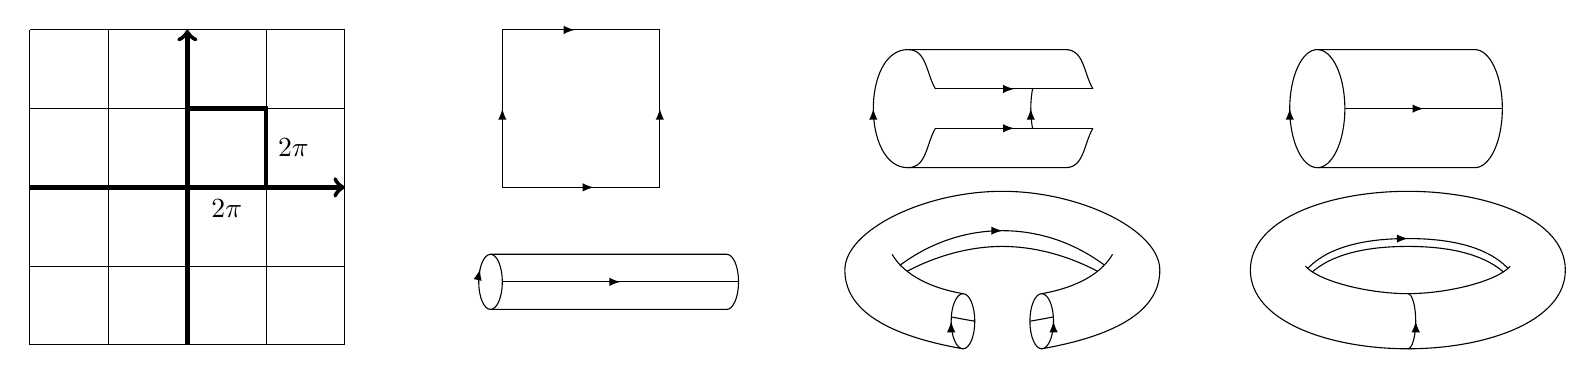
\begin{tikzpicture}
  % lattice
  \draw[->,ultra thick] (-2,0) -- (2,0);
  \draw[->,ultra thick] (0,-2) -- (0,2);
  \draw (-2,-2) grid (2,2);
  \node [draw,ultra thick,rectangle,minimum width=1cm,minimum height=1cm,label=below:$2 \pi$,label=right:$2 \pi$] at (0.5,0.5) {};

  % square
  \begin{scope}[xshift=4cm,yshift=1cm]
    \draw[postaction={decorate},decoration={
          markings,
          mark=at position .145 with {\arrow{latex}},
          mark=at position .375 with {\arrow{latex}},
          mark=at position .635 with {\arrowreversed{latex}},
          mark=at position .875 with {\arrowreversed{latex}},
        }
    ]
    (0,-1) -- +(2,0) -- +(2,2) -- +(0,2) -- cycle;
  \end{scope}

  % bracelet
  \begin{scope}[xshift=9.5cm,yshift=1cm]
    \draw[postaction={decorate},decoration={
          markings,
          mark=at position .5 with {\arrow{latex}}
        }
    ]
    (0,.25) -- ++(2,0);
    \draw[postaction={decorate},decoration={
          markings,
          mark=at position .5 with {\arrow{latex}}
        }
    ]
    (0,-.25) -- ++(2,0);
    \draw[postaction={decorate},decoration={
          markings,
          mark=at position .5 with {\arrow{latex}},
        }
    ] (0,-.25) to[out=-120,in=0] (-.35,-.75) to[out=180,in=180] (-.35,.75) to[out=0,in=120] (0,.25);
    \draw (2,.25) to[out=120,in=0] (1.65,.75) -- (-.35,.75) (-.35,-.75) -- (1.65,-.75) to[out=0,in=-120] (2,-.25);
    \begin{scope}
      \clip (0,.25) rectangle (2,-.25);
      \draw[postaction={decorate},decoration={
            markings,
            mark=at position .5 with {\arrowreversed{latex}},
          }
      ] (1.65,.75) to[out=180,in=180] (1.65,-.75);
    \end{scope}
  \end{scope}

  % cylinder
  \begin{scope}[xshift=14.7cm,yshift=1cm]
    \draw[postaction={decorate},decoration={
          markings,
          mark=at position .5 with {\arrow{latex}},
        }
    ] (0,0) -- (2,0);
    \draw[postaction={decorate},decoration={
          markings,
          mark=at position .5 with {\arrow{latex}},
        }
    ] (0,0) arc[start angle=0,delta angle=-360,x radius=.35,y radius=.75];
    \draw (2,0) arc[start angle=0,delta angle=-90,x radius=.35,y radius=.75] -- ++(-2,0);
    \draw (2,0) arc[start angle=0,delta angle=90,x radius=.35,y radius=.75] -- ++(-2,0);
  \end{scope}

  % long cylinder
  \begin{scope}[xshift=4cm,yshift=-1.2cm]
    \draw[postaction={decorate},decoration={
          markings,
          mark=at position .5 with {\arrow{latex}},
        }
    ] (0,0) -- (3,0);
    \draw[postaction={decorate},decoration={
          markings,
          mark=at position .6 with {\arrow{latex}},
        }
    ] (0,0) arc[start angle=0,delta angle=-360,x radius=.15,y radius=.35];
    \draw (3,0) arc[start angle=0,delta angle=-90,x radius=.15,y radius=.35] -- ++(-3,0);
    \draw (3,0) arc[start angle=0,delta angle=90,x radius=.15,y radius=.35] -- ++(-3,0);
  \end{scope}

  % open torus
  \begin{scope}[xshift=9cm,yshift=-1.7cm]
    \draw[postaction={decorate},decoration={
          markings,
          mark=at position .5 with {\arrow{latex}},
        }
    ] (1,0) arc[start angle=0,delta angle=-360,x radius=.15,y radius=.35];
    \draw (1,0) ++(-.15,-.35) .. controls +(170:1) and +(-90:.5) .. ++(-1.5,1) .. controls +(90:.5) and +(180:1) .. ++(2,1) .. controls +(0:1) and +(90:.5) .. ++(2,-1) .. controls +(-90:.5) and +(10:1) .. ++(-1.5,-1) coordinate (a);
    \draw[postaction={decorate},decoration={
          markings,
          mark=at position .5 with {\arrow{latex}},
        }
    ] (a) ++(-.15,.35) arc[start angle=0,delta angle=-360,x radius=-.15,y radius=.35];
    \draw (1,0) ++(-.15,.35) .. controls +(170:.5) and +(-60:.25) .. ++(-.9,.5) coordinate (b);
    \draw (a) ++(0,.7) .. controls +(10:.5) and +(240:.25) .. ++(.9,.5) coordinate (c);
    \begin{scope}
      \clip (1,0) ++(-.15,.35) .. controls +(170:.5) and +(-60:.25) .. ++(-.9,.5) -- ++(0,2) -| (c) .. controls +(240:.25) and +(10:.5) .. ++(-.9,-.5);
      \draw (1,0) ++(-.15,-.35) ++(0,-.7) .. controls +(170:1) and +(-90:.5) .. ++(-1.5,.8) .. controls +(90:.5) and +(180:1) .. ++(2,1.2) .. controls +(0:1) and +(90:.5) .. ++(2,-1.2) .. controls +(-90:.5) and +(10:1) .. ++(-1.5,-.8);
      \draw[postaction={decorate},decoration={
            markings,
            mark=at position .5 with {\arrow{latex}},
          }
      ] (1,0) ++(-.15,-.35) ++(0,-.8) .. controls +(170:1) and +(-90:.5) .. ++(-1.5,.8) .. controls +(90:.5) and +(180:1.2) .. ++(2,1.5) .. controls +(0:1.2) and +(90:.5) .. ++(2,-1.5) .. controls +(-90:.5) and +(10:1) .. ++(-1.5,-.8);
    \end{scope}
    \begin{scope}
      \clip (a) ++(-.15,.35) arc[start angle=0,delta angle=-360,x radius=-.15,y radius=.35];
      \draw (a) ++(-.15,.35) .. controls +(10:1) and +(-90:.5) .. ++(1.5,.8);
    \end{scope}
    \begin{scope}
      \clip (1,0) arc[start angle=0,delta angle=-360,x radius=.15,y radius=.35];
      \draw (1,0) .. controls +(170:1) and +(-90:.5) .. ++(-1.5,.8);
    \end{scope}
  \end{scope}

  % torus
  \begin{scope}[xshift=14cm,yshift=-1.7cm]
    \draw[postaction={decorate},decoration={
          markings,
          mark=at position .5 with {\arrowreversed{latex}},
        }
    ] (1.5,.35) arc[start angle=90,end angle=-90,y radius=.35,x radius=.1];
    \draw (1.5,-.35) .. controls +(180:1) and +(-90:.65) .. ++(-2,1) .. controls +(90:.65) and +(180:1) .. ++(2,1) .. controls +(0:1) and +(90:.65) .. ++(2,-1) .. controls +(-90:.65) and +(0:1) .. ++(-2,-1); \draw (1.5,.35) .. controls +(180:.5) and +(-50:.25) .. ++(-1.3,.35) coordinate (b);
    \draw (1.5,.35) .. controls +(0:.5) and +(230:.25) .. ++(1.3,.35) coordinate (c);
    \begin{scope}
      \clip (1.5,.35) .. controls +(180:.5) and +(-50:.25) .. ++(-1.3,.35) -- ++(0,2) -| (c) .. controls +(230:.25) and +(0:.5) .. ++(-1.3,-.35);
      \draw (1.5,-.35) ++(0,-.7) .. controls +(180:1) and +(-90:.65) .. ++(-1.5,1) .. controls +(90:.65) and +(180:1) .. ++(1.5,1) .. controls +(0:1) and +(90:.65) .. ++(1.5,-1) .. controls +(-90:.65) and +(0:1) .. ++(-1.5,-1);
      \draw[postaction={decorate},decoration={
            markings,
            mark=at position .5 with {\arrow{latex}},
          }
      ] (1.5,-.35) ++(0,-.6) .. controls +(180:1) and +(-90:.65) .. ++(-1.5,1) .. controls +(90:.65) and +(180:1) .. ++(1.5,1) .. controls +(0:1) and +(90:.65) .. ++(1.5,-1) .. controls +(-90:.65) and +(0:1) .. ++(-1.5,-1);
    \end{scope}
  \end{scope}

\end{tikzpicture}
\end{document}
